\sectionbreak \section{ \standartTitleFont
  Модуль DataManipulator
}

\subsection{ \standartTitleFont
  Назначение модуля DataManipulator
}

{\standartFont

  \par Модуль DataManipulator предназначен для различного рода обработки данных, с целью получения наборов данных (датасетов) необходимых для обучения моделей неройнных сетей. DataManipulator помогает преодолеть этап анализа и обработки данных, а также этап конструирования признаков.

  \par
}

\subsection{ \standartTitleFont
  Главное меню модуля DataManipulator.
}

{\standartFont

  \par В главном меню модуля DataManipulator представлены основные направления для обработки данных. Предоставляется выбор, с каким форматом данных будет происходить работа: с OCDF- или TDF-форматом. В главном меню также можно выбрать пункт, позволяющий создать TDF-данные на основе OCDF-данных. Также имеется пункт, который выводит на экран краткую информацию о форматах данных и о самом модуле DataManipulator. Внешний вид меню можно увидеть на рисунке \ref{fig:mainMenu}

  \par

  \begin{figure}[H]
    \centering
    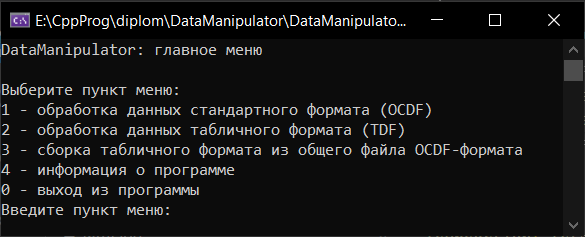
\includegraphics{images/forDataManipulator/mainMenu.png}
    \caption{главное меню модуля DataManipulator}
    \label{fig:mainMenu}
  \end{figure}

}

\subsection{ \standartTitleFont
  Меню обработки данных OCDF-формата модуля DataManipulator.
} 

\subsubsection{ \standartTitleFont
  Считывание OCDF-данных из файла.
} 

{\standartFont

  \par Для того, чтобы попасть в меню по обработке данных OCDF-формата будет предложено для начала их загрузить из файла. Это показано на рисунке на рисунке \ref{fig:readOCDFst1}.

  \begin{figure}[H]
    \centering
    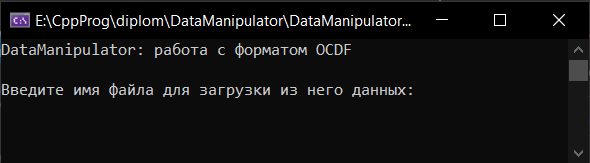
\includegraphics[width=\textwidth]{images/forDataManipulator/readOCDFstage1.png}
    \caption{указание файла для загрузки из него OCDF-данных.}
    \label{fig:readOCDFst1}
  \end{figure}

  \par Вводим путь к файлу или перетаскиваем файл в консоль для получения его абсолютного пути и нажимаем Enter. После этого будет предложено ввести количество данных, которые необходимо считать из файла. Это показано на рисунке \ref{fig:readOCDFst2}.

  \begin{figure}[H]
    \centering
    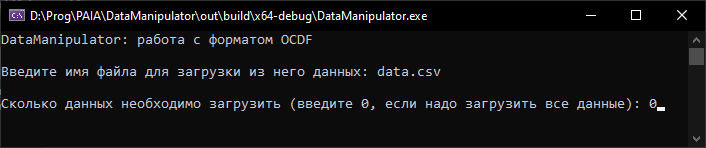
\includegraphics[width=\textwidth]{images/forDataManipulator/readOCDFstage2.png}
    \caption{указание необходимого количества данных для считывания.}
    \label{fig:readOCDFst2}
  \end{figure}

  \par Есть несколько особенностей, при вводе количества данных. В случае, если будет введён 0 или число, превышающее количество данных в файле, то будут считаны все данные, которые есть в файле. Если будет введено отрицательное число или хотя бы один символ, отличный от цифр, то программа выдаст предупреждение о некорректном вводе данных, показанное на рисунке \ref{fig:readOCDFerror1}, и предложит ввести путь к файлу и необходимое количество данных для считывания снова. 

  \begin{figure}[H]
    \centering
    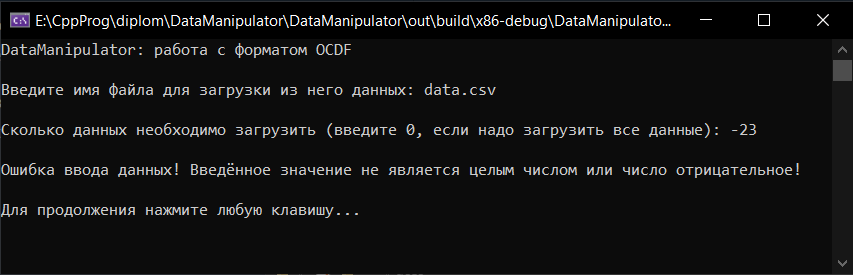
\includegraphics[width=\textwidth]{images/forDataManipulator/readOCDFerror1.png}
    \caption{предупреждение об ошибке при вводе необходимого количества данных для считывания.}
    \label{fig:readOCDFerror1}
  \end{figure}

  \par Могут возникнуть и другие предупреждения, связанные непосредственно с самим файлом. Если файл с данными не существует, или этот файл пуст, или данные в нём не представленны в необходимом формате, то возникнет предупреждение о невозможности чтения данных, представленное на рисунке \ref{fig:readOCDFerror2}.

  \begin{figure}[H]
    \centering
    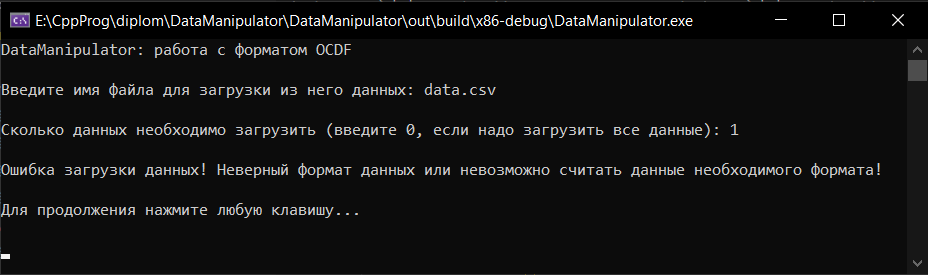
\includegraphics[width=\textwidth]{images/forDataManipulator/readOCDFerror2.png}
    \caption{предупреждение об ошибке чтения данных.} 
    \label{fig:readOCDFerror2}
  \end{figure}

  \par Как уже понятно, чтение данных происходит в текстовом режиме. Однако существует возможность считывать данные, которые представлены в бинарном виде. Для этого необходимо, чтобы файл имел расширение .bin, иначе чтение данных будет происходить в текстовом режиме. Пример файла с данными в бинарном виде можно увидеть на рисунке \ref{fig:readOCDFbin}.

  \begin{figure}[H]
    \centering
    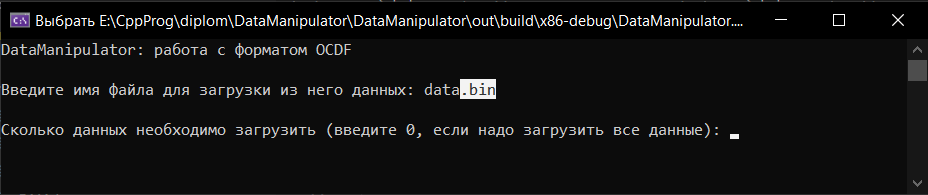
\includegraphics[width=\textwidth]{images/forDataManipulator/readOCDFbin.png}
    \caption{ввод файла с данными в бинарном виде.} 
    \label{fig:readOCDFbin}
  \end{figure}

  \par После указания файла с данными в бинарном виде будет предложено ввести количество данных, которое необходимо считать из файла. Все предупреждения, которые связаны с чтением данных и ввода значений уже разобраны выше. 

  \par
}

\subsubsection{ \standartTitleFont
  Возможности по обработке OCDF-данных. 
}

{\standartFont

  \par После считывания OCDF-данных из файла открывается меню для работы с данными, представленное на рисунке \ref{fig:OCDFmenu}.

  \begin{figure}[H]
    \centering
    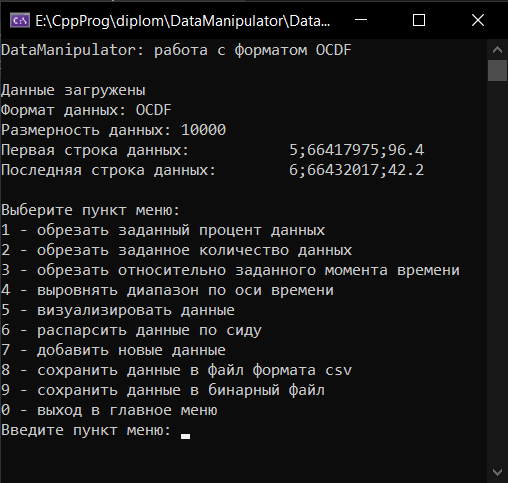
\includegraphics{images/forDataManipulator/OCDFmenu.png}
    \caption{ввод файла с данными в бинарном виде.} 
    \label{fig:OCDFmenu}
  \end{figure}

  \par В появившемся меню будет указана информация о считанных данных: формат данных, их количество, а также первая и последняя строки последовательности данных. После идёт выбор действий, которые можно совешить над данными: обрезка данных, визуализация данных, привидение данных к равноинтервальному виду, парсинг данных, добавление данных и сохранение результатов обработки. Каждое из них подробно будет разобрано ниже.

  \par
}

\subsection{ \standartTitleFont
  Обезка OCDF-данных. 
}

{\standartFont

  \par Существует 3 вида обрезки данных: обрезка заданного процента данных, обрезка заданного количества данных и обрезка по заданному моменту времени. Также у каждого вида обрезки данных существует 2 режима обрезки данных: обрезка данных слева направо или обрезка данных справо налево. Рассмотрим каждый вид обрезки данных на примерах данных, показанных на рисунке \ref{fig:ExOCDFdataForCating}. 

  \begin{figure}[H]
    \centering
    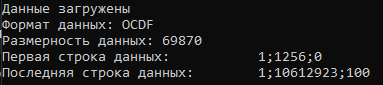
\includegraphics{images/forDataManipulator/ExOCDFdataForCating.png}
    \caption{пример данных для дальнейшей их обрезки.} 
    \label{fig:ExOCDFdataForCating}
  \end{figure}

  \par
}

\subsubsection{ \standartTitleFont
  Обрезка OCDF-данных по заданному проценту. 
}

{\standartFont

  \par Обрезка по заданному проценту данных оставляет введённое пользователем процентное количество данных от общего их количества. Для ввода процента обрезки данных необходимо задать число в промежутке (0,00; 1,00), где 0,00 - 0\%, а 1,00 - 100\%, как это показано на рисунке \ref{fig:OCDFcutper1}. 

  \begin{figure}[H]
    \centering
    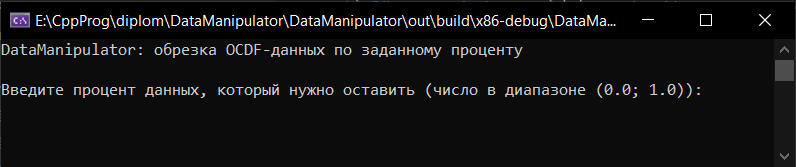
\includegraphics{images/forDataManipulator/OCDFcutpercentstage1.png}
    \caption{ввод процента для обрезки данных.} 
    \label{fig:OCDFcutper1}
  \end{figure}

  \par После ввода процента для обрезки данных, программа предлагает выбрать режим обрезки, введя значения 0 или 1, как показано на рисунке \ref{fig:OCDFcutper2}. 

  \begin{figure}[H]
    \centering
    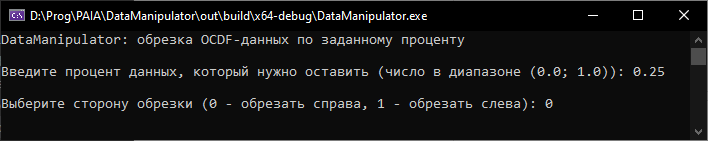
\includegraphics[width=\textwidth]{images/forDataManipulator/OCDFcutpercentstage2.png}
    \caption{ввод режима для обрезки по заданному проценту.} 
    \label{fig:OCDFcutper2}
  \end{figure}

  \par Если ввести 0, то заданный процент данных будет оставлен слева, т.е. в начале. Если ввести 1, то заданный процент данных будет оставлен справа, т.е. в конце. Вводим режим обрезки данных 0 и смотрим результаты на рисунке \ref{fig:ExOCDFdataAftCatPer}. 

  \begin{figure}[H]
    \centering
    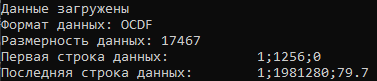
\includegraphics{images/forDataManipulator/ExOCDFdataAftCatPer.png}
    \caption{результаты обрезки данных по заданому проценту.} 
    \label{fig:ExOCDFdataAftCatPer}
  \end{figure}

  \par Была произведена обрезка 75\% данных от общего количества, поскольку было введён 25\% данных, которые необходимо оставить, в режиме справо налево, т.е. с конца. 

  \par 
}

\subsubsection{ \standartTitleFont
  Обрезка OCDF-данных по заданному количеству. 
}

{\standartFont

  \par Обрезка по заданному количеству данных оставляет введённое пользователем количество данных. Для ввода количества обрезки данных необходимо задать целое положительное число отличное от нуля, как это показано на рисунке \ref{fig:OCDFcutquan1}. 

  \begin{figure}[H]
    \centering
    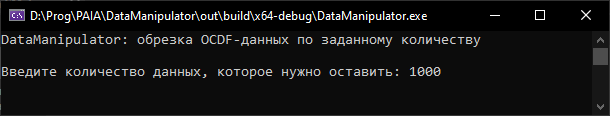
\includegraphics{images/forDataManipulator/OCDFcutquantitystage1.png}
    \caption{ввод значения количества для обрезки данных.} 
    \label{fig:OCDFcutquan1}
  \end{figure}

  \par После ввода количества для обрезки данных, программа предлагает выбрать режим обрезки, введя значения 0 или 1, как показано на рисунке \ref{fig:OCDFcutquan2}. 

  \begin{figure}[H]
    \centering
    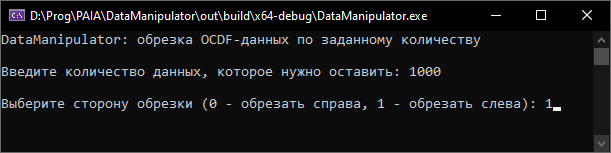
\includegraphics{images/forDataManipulator/OCDFcutquantitystage2.png}
    \caption{ввод режима для обрезки по заданному количеству.} 
    \label{fig:OCDFcutquan2}
  \end{figure}

  \par Если ввести 0, то заданное количество данных будет оставлено слева, т.е. в начале. Если ввести 1, то заданное количество данных будет оставлено справо, т.е. в конце. Вводим режим обрезки данных 1 и смотрим результаты на рисунке \ref{fig:ExOCDFdataAftCatQuan}. 

  \begin{figure}[H]
    \centering
    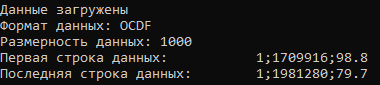
\includegraphics{images/forDataManipulator/ExOCDFdataAftCatQuan.png}
    \caption{результаты обрезки данных по заданому количеству.} 
    \label{fig:ExOCDFdataAftCatQuan}
  \end{figure}

  \par Была произведена обрезка 16467 данных, поскольку было введено 1000 данных, которые необходимо оставить, в режиме справо налево, т.е. в конце. 

  \par 
}

\subsubsection{ \standartTitleFont
  Обрезка OCDF-данных по заданному моменту времени. 
}

{\standartFont

  \par Обрезка по заданному моменту времени оставляет промежуток данных до или после указанного момента. Для ввода момента времени для обрезки данных необходимо задать целое положительное число отличное от нуля, как это показано на рисунке \ref{fig:OCDFcutmom1}. 

  \begin{figure}[H]
    \centering
    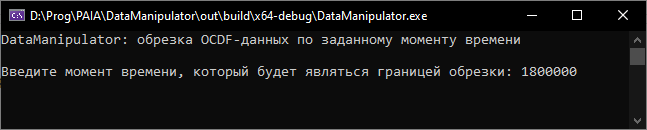
\includegraphics{images/forDataManipulator/OCDFcutmomentstage1.png}
    \caption{ввод значения момента времени для обрезки данных.} 
    \label{fig:OCDFcutmom1}
  \end{figure}

  \par После ввода момента времени для обрезки данных, программа предлагает выбрать режим обрезки, введя значения 0 или 1, как показано на рисунке \ref{fig:OCDFcutmom2}. 

  \begin{figure}[H]
    \centering
    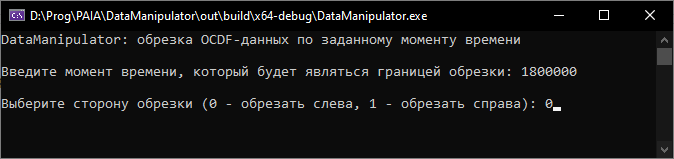
\includegraphics[width=\textwidth]{images/forDataManipulator/OCDFcutmomentstage2.png}
    \caption{ввод режима для обрезки по заданному моменту времени.} 
    \label{fig:OCDFcutmom2}
  \end{figure}

  \par Если ввести 0, то данные будут оставлены слева относительно заданного момента времени, т.е. в начале. Если ввести 1, то данные будут оставлены справа относительно заданного момента времени, т.е. в конце. Вводим режим обрезки данных 0 и смотрим результаты на рисунке \ref{fig:ExOCDFdataAftCatMom}. 

  \begin{figure}[H]
    \centering
    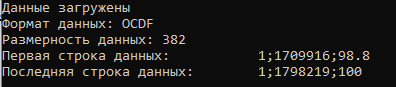
\includegraphics{images/forDataManipulator/ExOCDFdataAftCatMom.png}
    \caption{результаты обрезки данных по заданному моменту времени времени.} 
    \label{fig:ExOCDFdataAftCatMom}
  \end{figure}

  \par 
}

\subsubsection{ \standartTitleFont
  Возможные ошибки при обрезке OCDF-данных. 
}

{\standartFont

  \par При обрезке данных могут возникать различные ситуации, которые способны вызывать всяческие ошибки или исключительные случаи. Самым основным, что может вызвать ошибку, это некорректный ввод данных. Так, например, при обрезке данных по заданному проценту не допустимо вводить числа не принадлежащие диапазону (0,00; 1,00), хоть и ввод 1,00 доступен, однако при этом данные никак не изменятся. Ввод отрицательных или не целых чисел при обрезке по заданному моменту времени и по заданному количеству данных также вызывает ошибки некорректного ввода. Пример такой ошибки продемонстрирован на рисунке \ref{fig:ExOCDFdataCatErr1}.

  \begin{figure}[H]
    \centering
    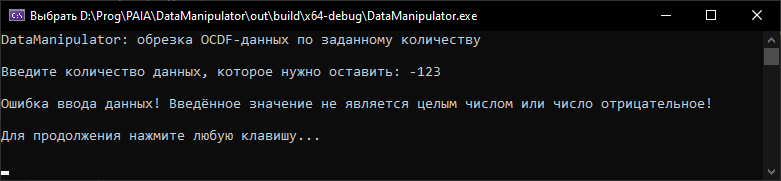
\includegraphics[width=\textwidth]{images/forDataManipulator/ExOCDFdataCatError1.png}
    \caption{пример ввода недопустимых чисел при обрезке OCDF-данных.} 
    \label{fig:ExOCDFdataCatErr1}
  \end{figure}

  \par Также может быть вызвана ошибка некоректного ввода, при использовании символов, отличных от цифр, характерное для всех видов обрезки. Пример такой ошибки продемонстрирован на рисунке \ref{fig:ExOCDFdataCatErr2}.

  \begin{figure}[H]
    \centering
    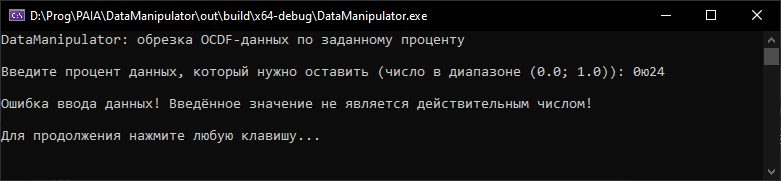
\includegraphics[width=\textwidth]{images/forDataManipulator/ExOCDFdataCatError2.png}
    \caption{пример ввода недопустимых символов при обрезке OCDF-данных.} 
    \label{fig:ExOCDFdataCatErr2}
  \end{figure}

  \par При обрезке данных по заданному количеству есть вероятность того, что пользователь введёт число больше общего количества данных. В таком случае данные не изменятся и ошибка не появится. 

  \par При обрезке данных по заданному моменту времени есть вероятность того, что пользователь введёт момент времени, который находится раньше начального момента вермени или позже конечного момента времени в самих данных. В таком случае, если будет выбран соотвествующий режим обрезки, данные либо никак не изменятся, либо появится ошибка о возврате пустых данных, что продемонстрирована на рисунке \ref{fig:ExOCDFdataCatErr3}.

  \begin{figure}[H]
    \centering
    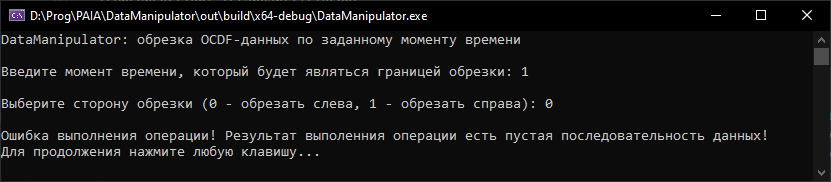
\includegraphics[width=\textwidth]{images/forDataManipulator/ExOCDFdataCatError3.png}
    \caption{пример ошибки при возврате пустых OCDF-данных.} 
    \label{fig:ExOCDFdataCatErr3}
  \end{figure}

  \par Такая ошибка может возникать также при вводе 0,00 для обрезки данных по заданному проценту. В случае такой ошибки данные никак не изменятся и управление перейдёт к меню обработки OCDF-данных.
  
  \par Последняя возможная ошибка относится к вводу недопустимых символов при выборе режимов обрезки. В таком случае возникает ошибка, которая перезапускает операцию заново. Пример такой ошибки продемонстрирован на рисунке \ref{fig:ExOCDFdataCatErr4}.

  \begin{figure}[H]
    \centering
    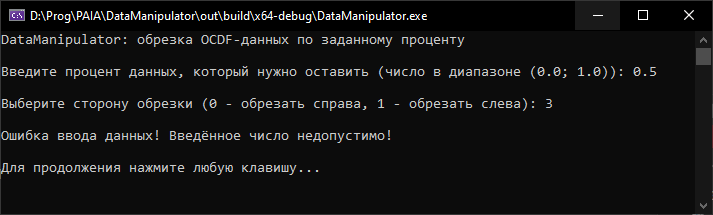
\includegraphics[width=\textwidth]{images/forDataManipulator/ExOCDFdataCatError4.png}
    \caption{пример ввода некоретных данных при выборе режима обрезки OCDF-данных.} 
    \label{fig:ExOCDFdataCatErr4}
  \end{figure}

  \par
}

\subsection{ \standartTitleFont
  Парсинг OCDF-данных. 
}

{\standartFont

  \par Основной функцией парсинга данных является разделение данных относительно указанного сида для данных, где имеются значения двух и более сидов, с целью получения данных, содержащих информацию, относящуюся исключительно к указанному сиду.

  \par 
}

\subsubsection{ \standartTitleFont
  Процесс парсинга OCDF-данных. 
}

{\standartFont

  \par Процесс парсинга начинается с того, что программа запрашивает: данные какого сида необходимо получить? Это можно увидеть на рисунке \ref{fig:OCDFdataParsSt}.

  \begin{figure}[H]
    \centering
    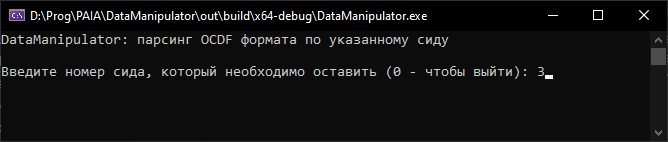
\includegraphics[width=\textwidth]{images/forDataManipulator/OCDFdataParcing.png}
    \caption{ввод номера сида для парсинга OCDF-данных.} 

    \label{fig:OCDFdataParsSt}
  \end{figure}

  \par После ввода номера сида, который необходимо получить, выполняется сам процесс парсинга, результатом которого являются данные, содержащие информацию, касающиеся указанного сида. Данная операция весьма проста.

  \par 
}

\subsubsection{ \standartTitleFont
  Возможные ошибки при парсинге OCDF-данных.
}

{\standartFont

  \par Несмотря на простоту операции парсинга, всей же есть ситуации, при которых возникают ошибки или исключительные случаи. 

  \par Ошибка может возникать, если ввести недопустимый сид. На данный момент программа считает допустимыми следующие сиды: 1, 2, 3, 4, 5, 6. Иные введёные числа вызывают ошибку, продемонстрированную на рисунке \ref{fig:OCDFdataParsErrUnkcid}.

  \begin{figure}[H]
    \centering
    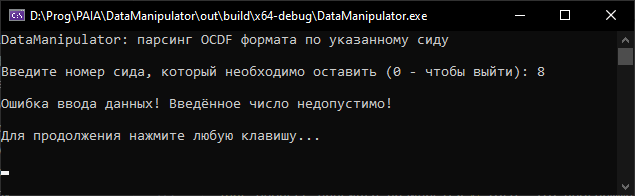
\includegraphics{images/forDataManipulator/OCDFdataParsErrUnknowCID.png}
    \caption{ошибка ввода несуществующего сида при парсинге OCDF-данных.} 
    \label{fig:OCDFdataParsErrUnkcid}
  \end{figure}

  \par Ошибка также может возникать, если ввести недопустимые символы, т.е. символы отличные от цифр. Данная ошибка продемонстрирована на рисунке \ref{fig:OCDFdataParsErrInv}.

  \begin{figure}[H]
    \centering
    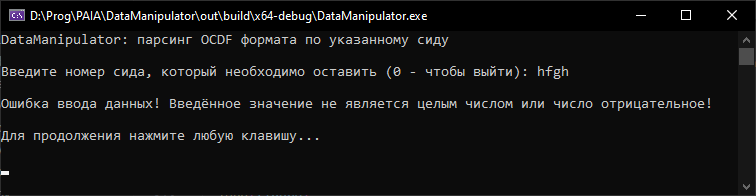
\includegraphics[width=\textwidth]{images/forDataManipulator/OCDFdataParsErrInvalid.png}
    \caption{ошибка ввода недопустимого символа при парсинге OCDF-данных.} 
    \label{fig:OCDFdataParsErrInv}
  \end{figure}

  \par Также ошибка может возникать в случае, если был введён сид, которого нет в данных, подвергаемых парсингу. Данная ошибка продемонстрирована на рисунке \ref{fig:OCDFdataParsErrnotcid}.

  \begin{figure}[H]
    \centering
    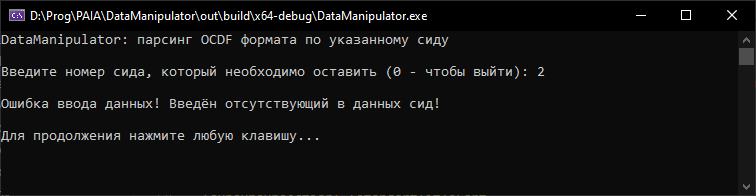
\includegraphics[width=\textwidth]{images/forDataManipulator/OCDFdataParsErrNotCID.png}
    \caption{ошибка ввода отсутствующего сида в OCDF-данных.} 
    \label{fig:OCDFdataParsErrnotcid}
  \end{figure}

  \par Результатом выше перечисленных ошибок будет перезапуск операции парсинга. 

}

\subsection{ \standartTitleFont
  Выравнивание диапазонов OCDF-данных.
}

\subsubsection{ \standartTitleFont
  Математические основы выравнивания диапазонов OCDF-данных.
}

\subsubsection{ \standartTitleFont
  Процесс выравнивания диапазонов OCDF-данных.
}

\subsubsection{ \standartTitleFont
  Возможные ошибки при выравнивании диапазонов OCDF-данных.
}

\subsection{ \standartTitleFont
  Сохранение OCDF-данных в файл формата csv.
}

\subsection{ \standartTitleFont
  Сохранение OCDF-данных в бинарный файл.
}